% MSc dissertation example file, February 2022
%
% Leave one of the documentclass lines uncommented to match your degree.
% You may remove the logo option if it causes problems.
% Do not change any other options.
% \documentclass[logo,msc,adi]{infthesis}     % Adv Design Inf
% \documentclass[logo,msc,ai]{infthesis}      % AI
% \documentclass[logo,msc,cogsci]{infthesis}  % Cognitive Sci
% \documentclass[logo,msc,cs]{infthesis}      % Computer Sci
% \documentclass[logo,msc,cyber]{infthesis}   % Cyber Sec
% \documentclass[logo,msc,datasci]{infthesis} % Data Sci
% \documentclass[logo,msc,di]{infthesis}      % Design Inf
% \documentclass[logo,msc,dsti]{infthesis}    % Data Sci TI
% \documentclass[logo,msc,inf]{infthesis}     % Informatics
\documentclass[logo,msc]{infthesis}           % degree unspecified, do not change except to add your degree
%%%%%%%%%%%%%%%%%%%%%%%%
% Understand any problems and seek approval before assuming it's ok to remove ugcheck.
\usepackage{msccheck}

% Include any packages you need below, but don't include any that change the page
% layout or style of the dissertation. By including the ugcheck package above,
% you should catch most accident-al changes of page layout though.
%\documentclass{article}
\usepackage{mathtools}
\usepackage{microtype} % recommended, but you can remove if it causes problems
\usepackage{graphicx}
\usepackage{subfig}
\usepackage{algorithm}
\usepackage[lined,boxed,linesnumbered]{algorithm2e}
\usepackage{algpseudocode}


\begin{document}
\begin{preliminary}

\title{Machine Learning of Polyhedral Compilation}

\author{Prakshal Nandi}

\date{\today}



\chapter{Results}

Starategies:

Simple : Simple Representation

Full : Full Representation with all information

Std: Standardisation applied to features

NoStd : No Standardisation applied to features

Bias : Bias introduced while selecting coeffiecients (coeff0)

NoBias : No Bias introduced.

\begin{figure}
\centering
\begin{minipage}{.45\linewidth}
  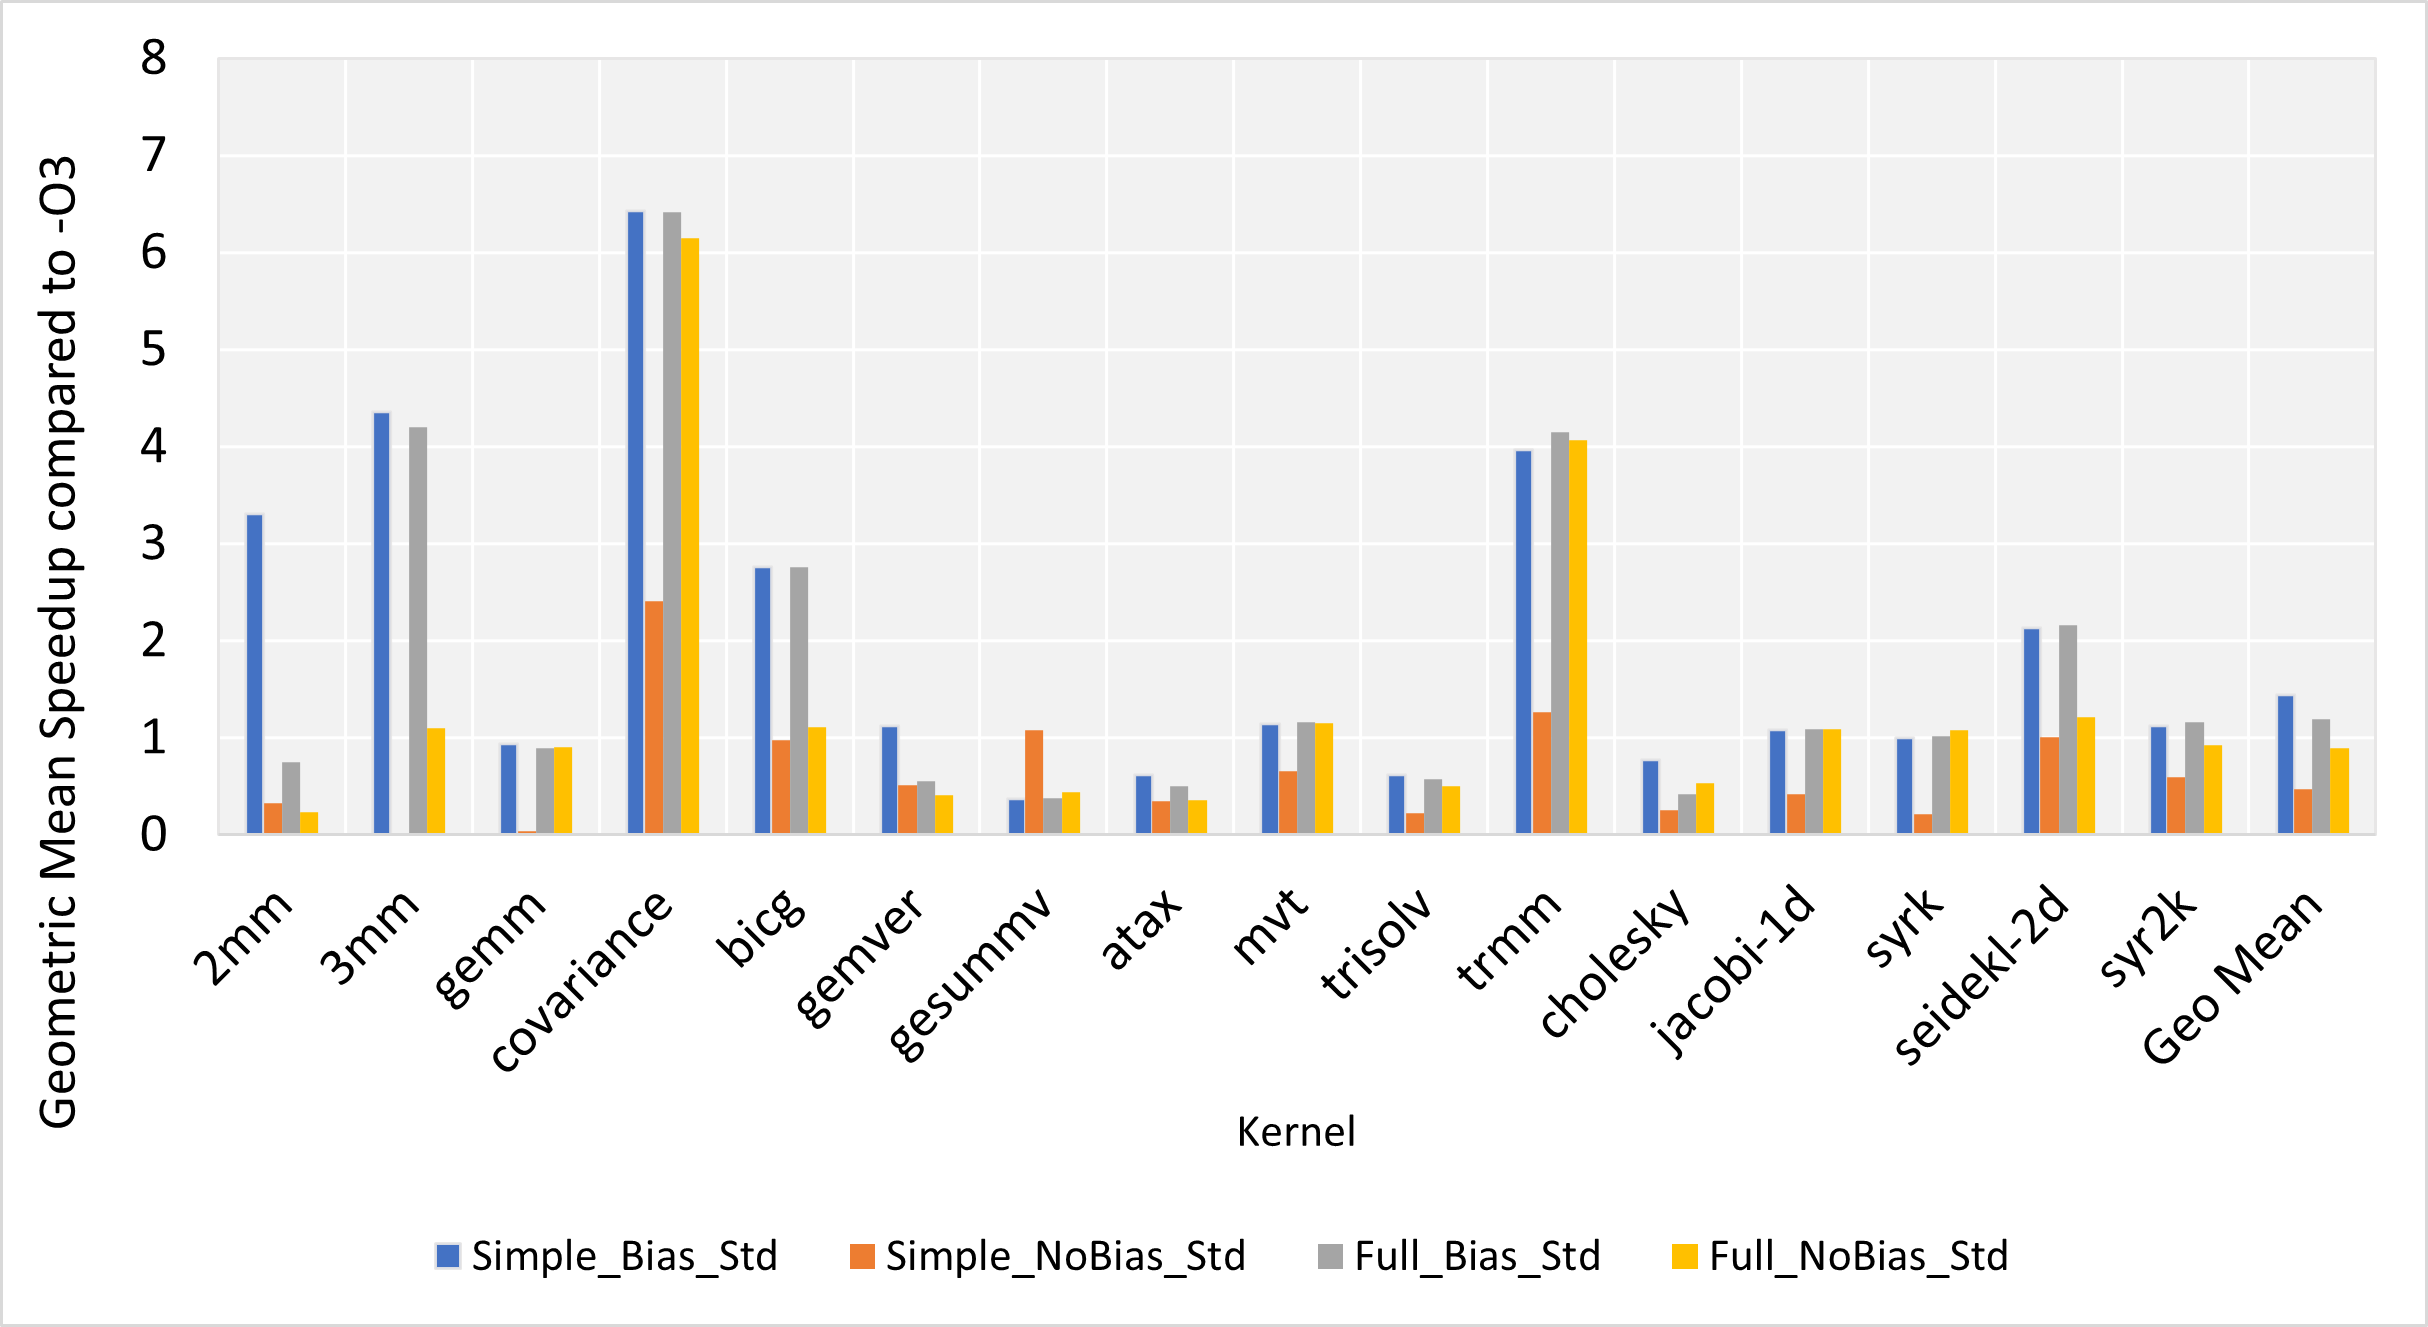
\includegraphics[width=\linewidth]{Images/Std_Chart.png}
  \captionof{figure}{With Standardisation}
  \label{Std_Chart}
\end{minipage}
\hspace{.05\linewidth}
\begin{minipage}{.45\linewidth}
  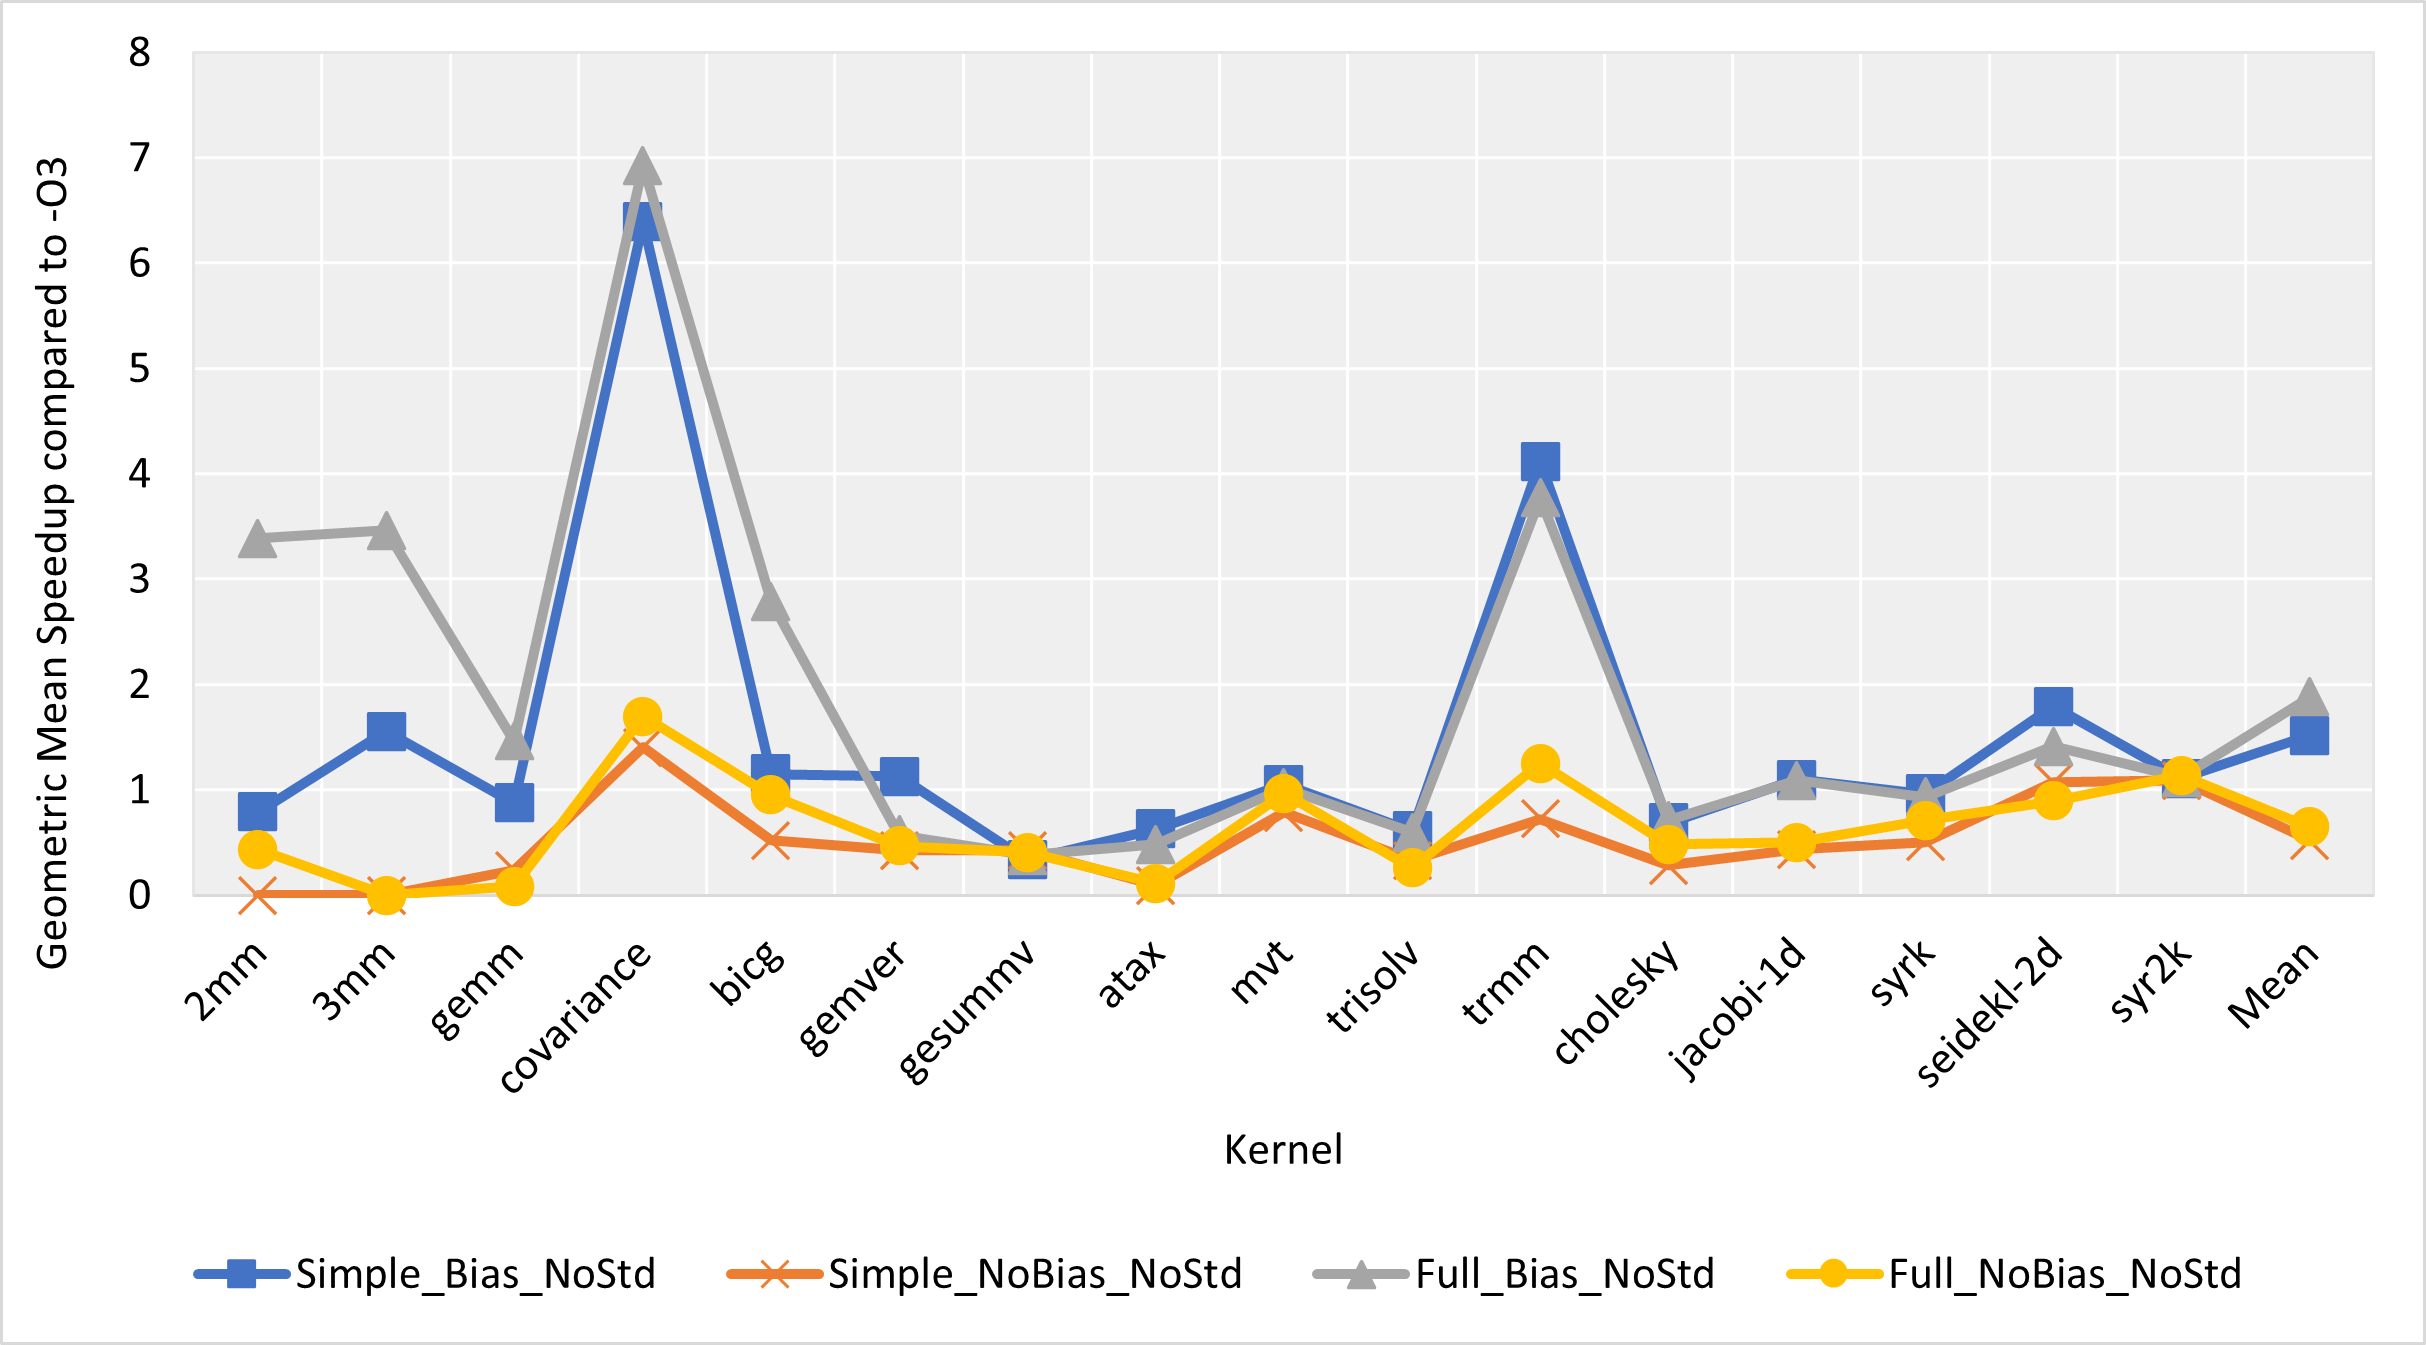
\includegraphics[width=\linewidth]{Images/NoStd_Chart.png}
  \captionof{figure}{Without Standardisation}
  \label{NoStd_Chart}
\end{minipage}
\State{Comparison of PolyGymRL Results for Standardisation and No Standardisation Approach}
\end{figure}

\begin{figure}
\centering
\begin{minipage}{.45\linewidth}
  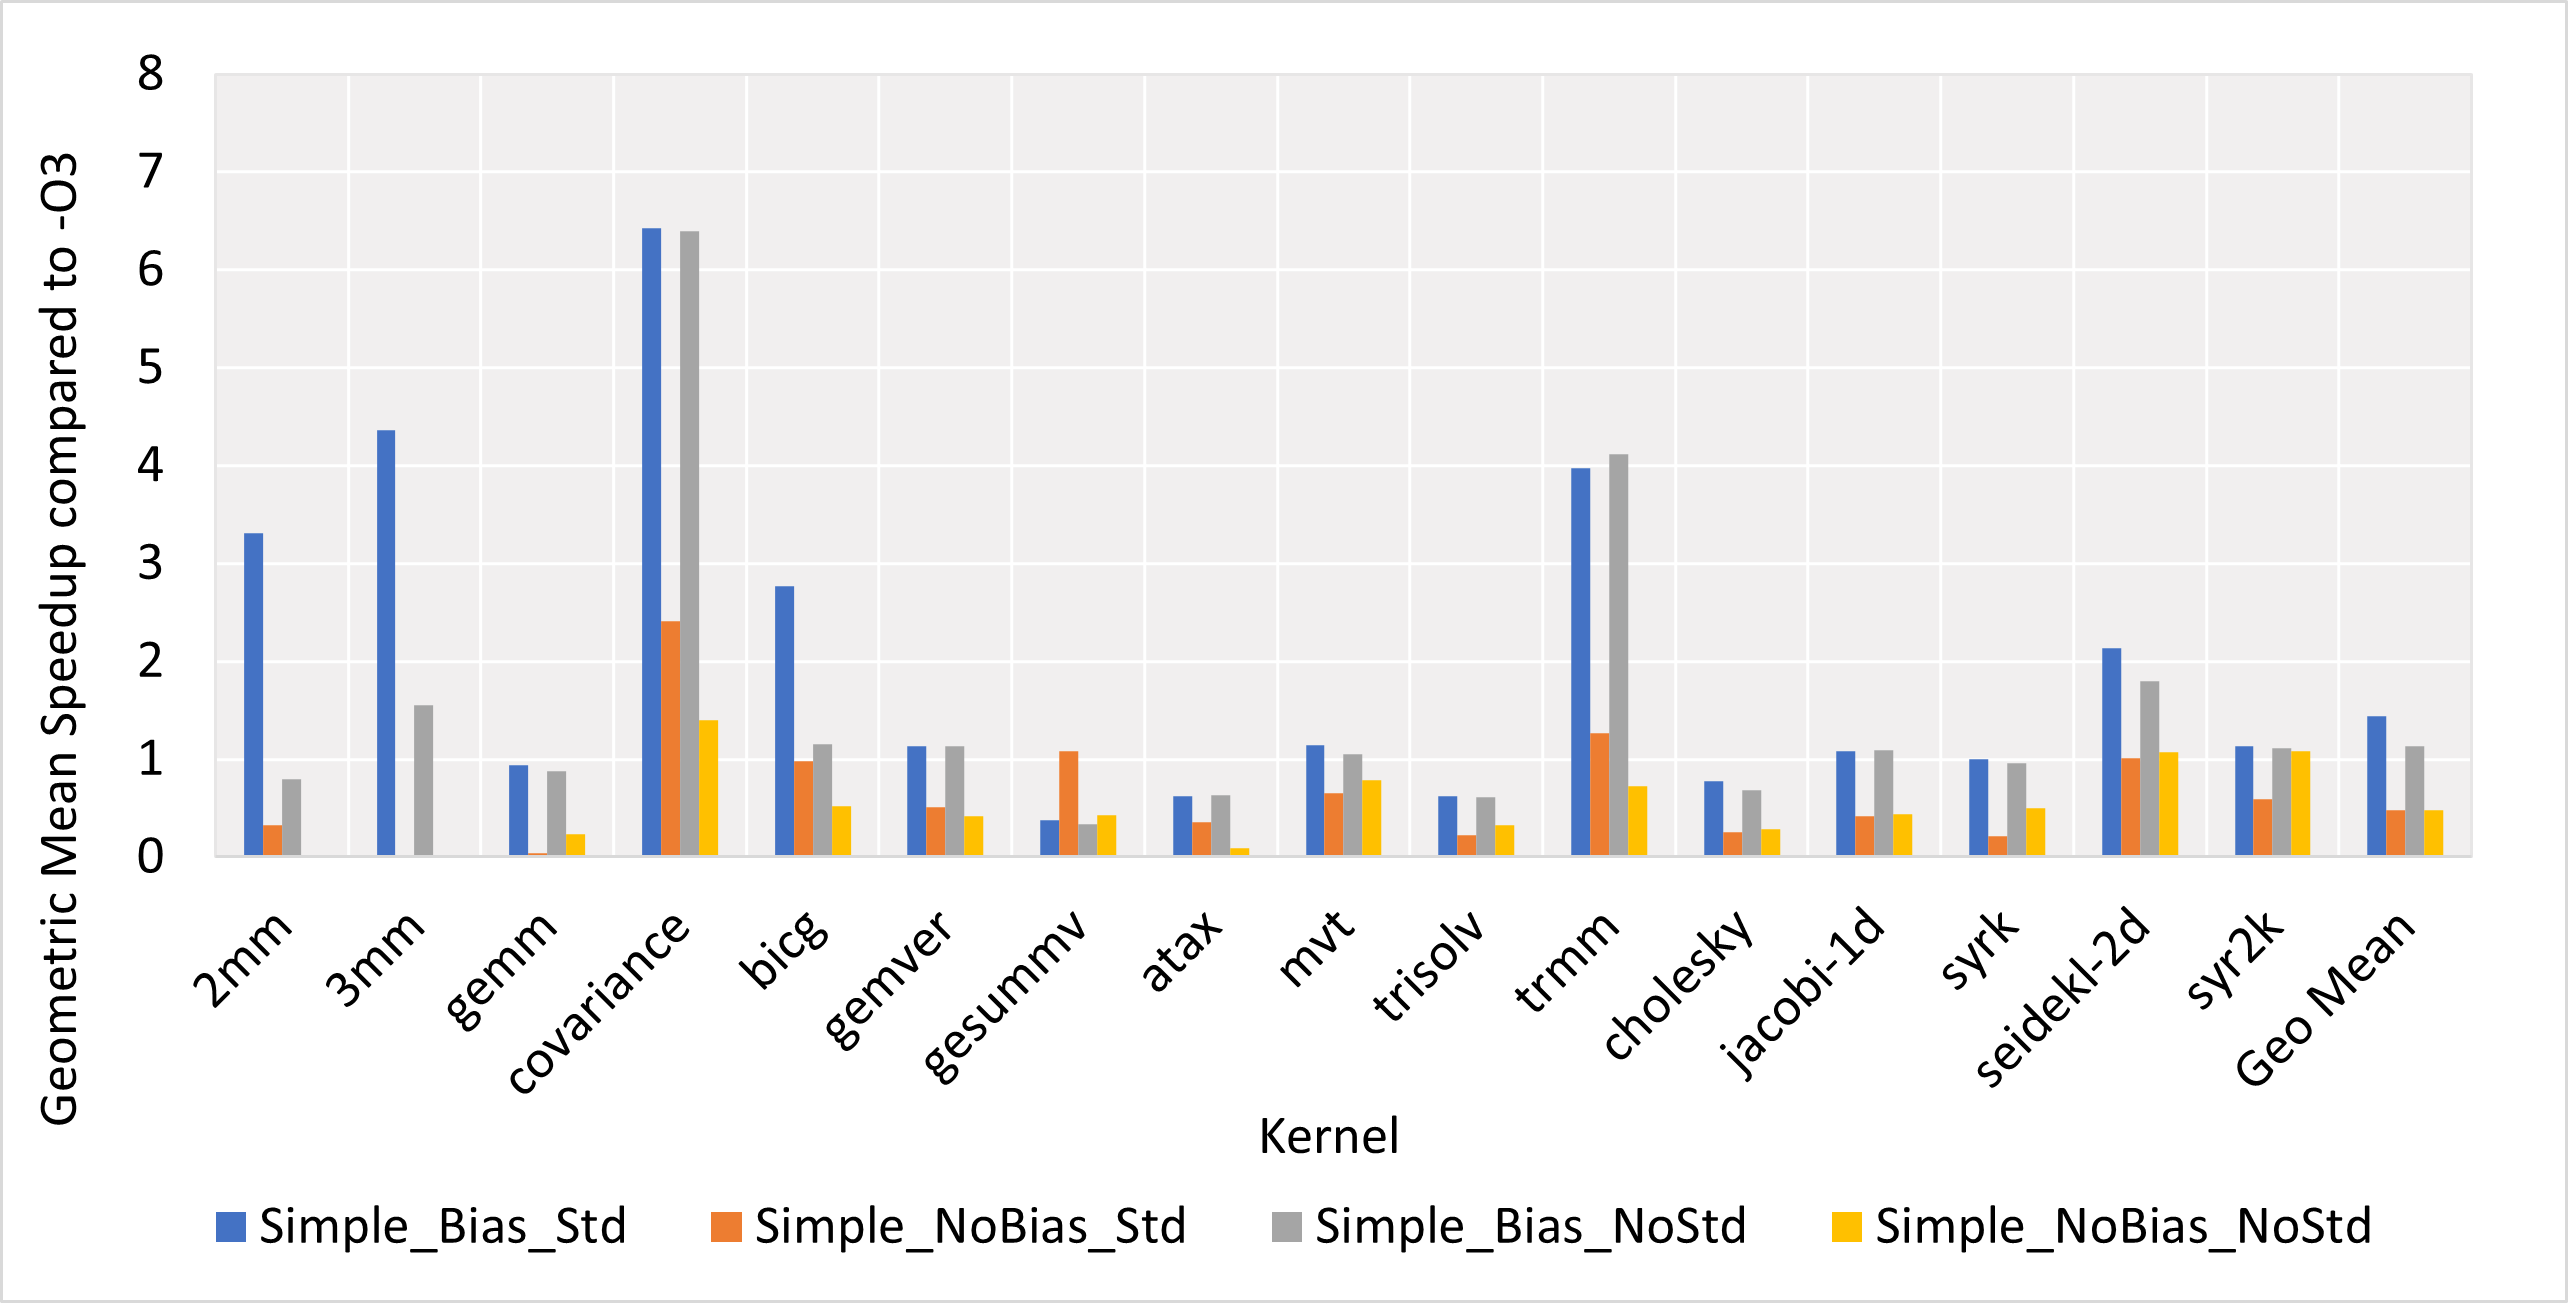
\includegraphics[width=\linewidth]{Images/Simple_Chart.png}
  \captionof{figure}{Simple Representation}
  \label{Simple_Chart}
\end{minipage}
\hspace{.05\linewidth}
\begin{minipage}{.45\linewidth}
  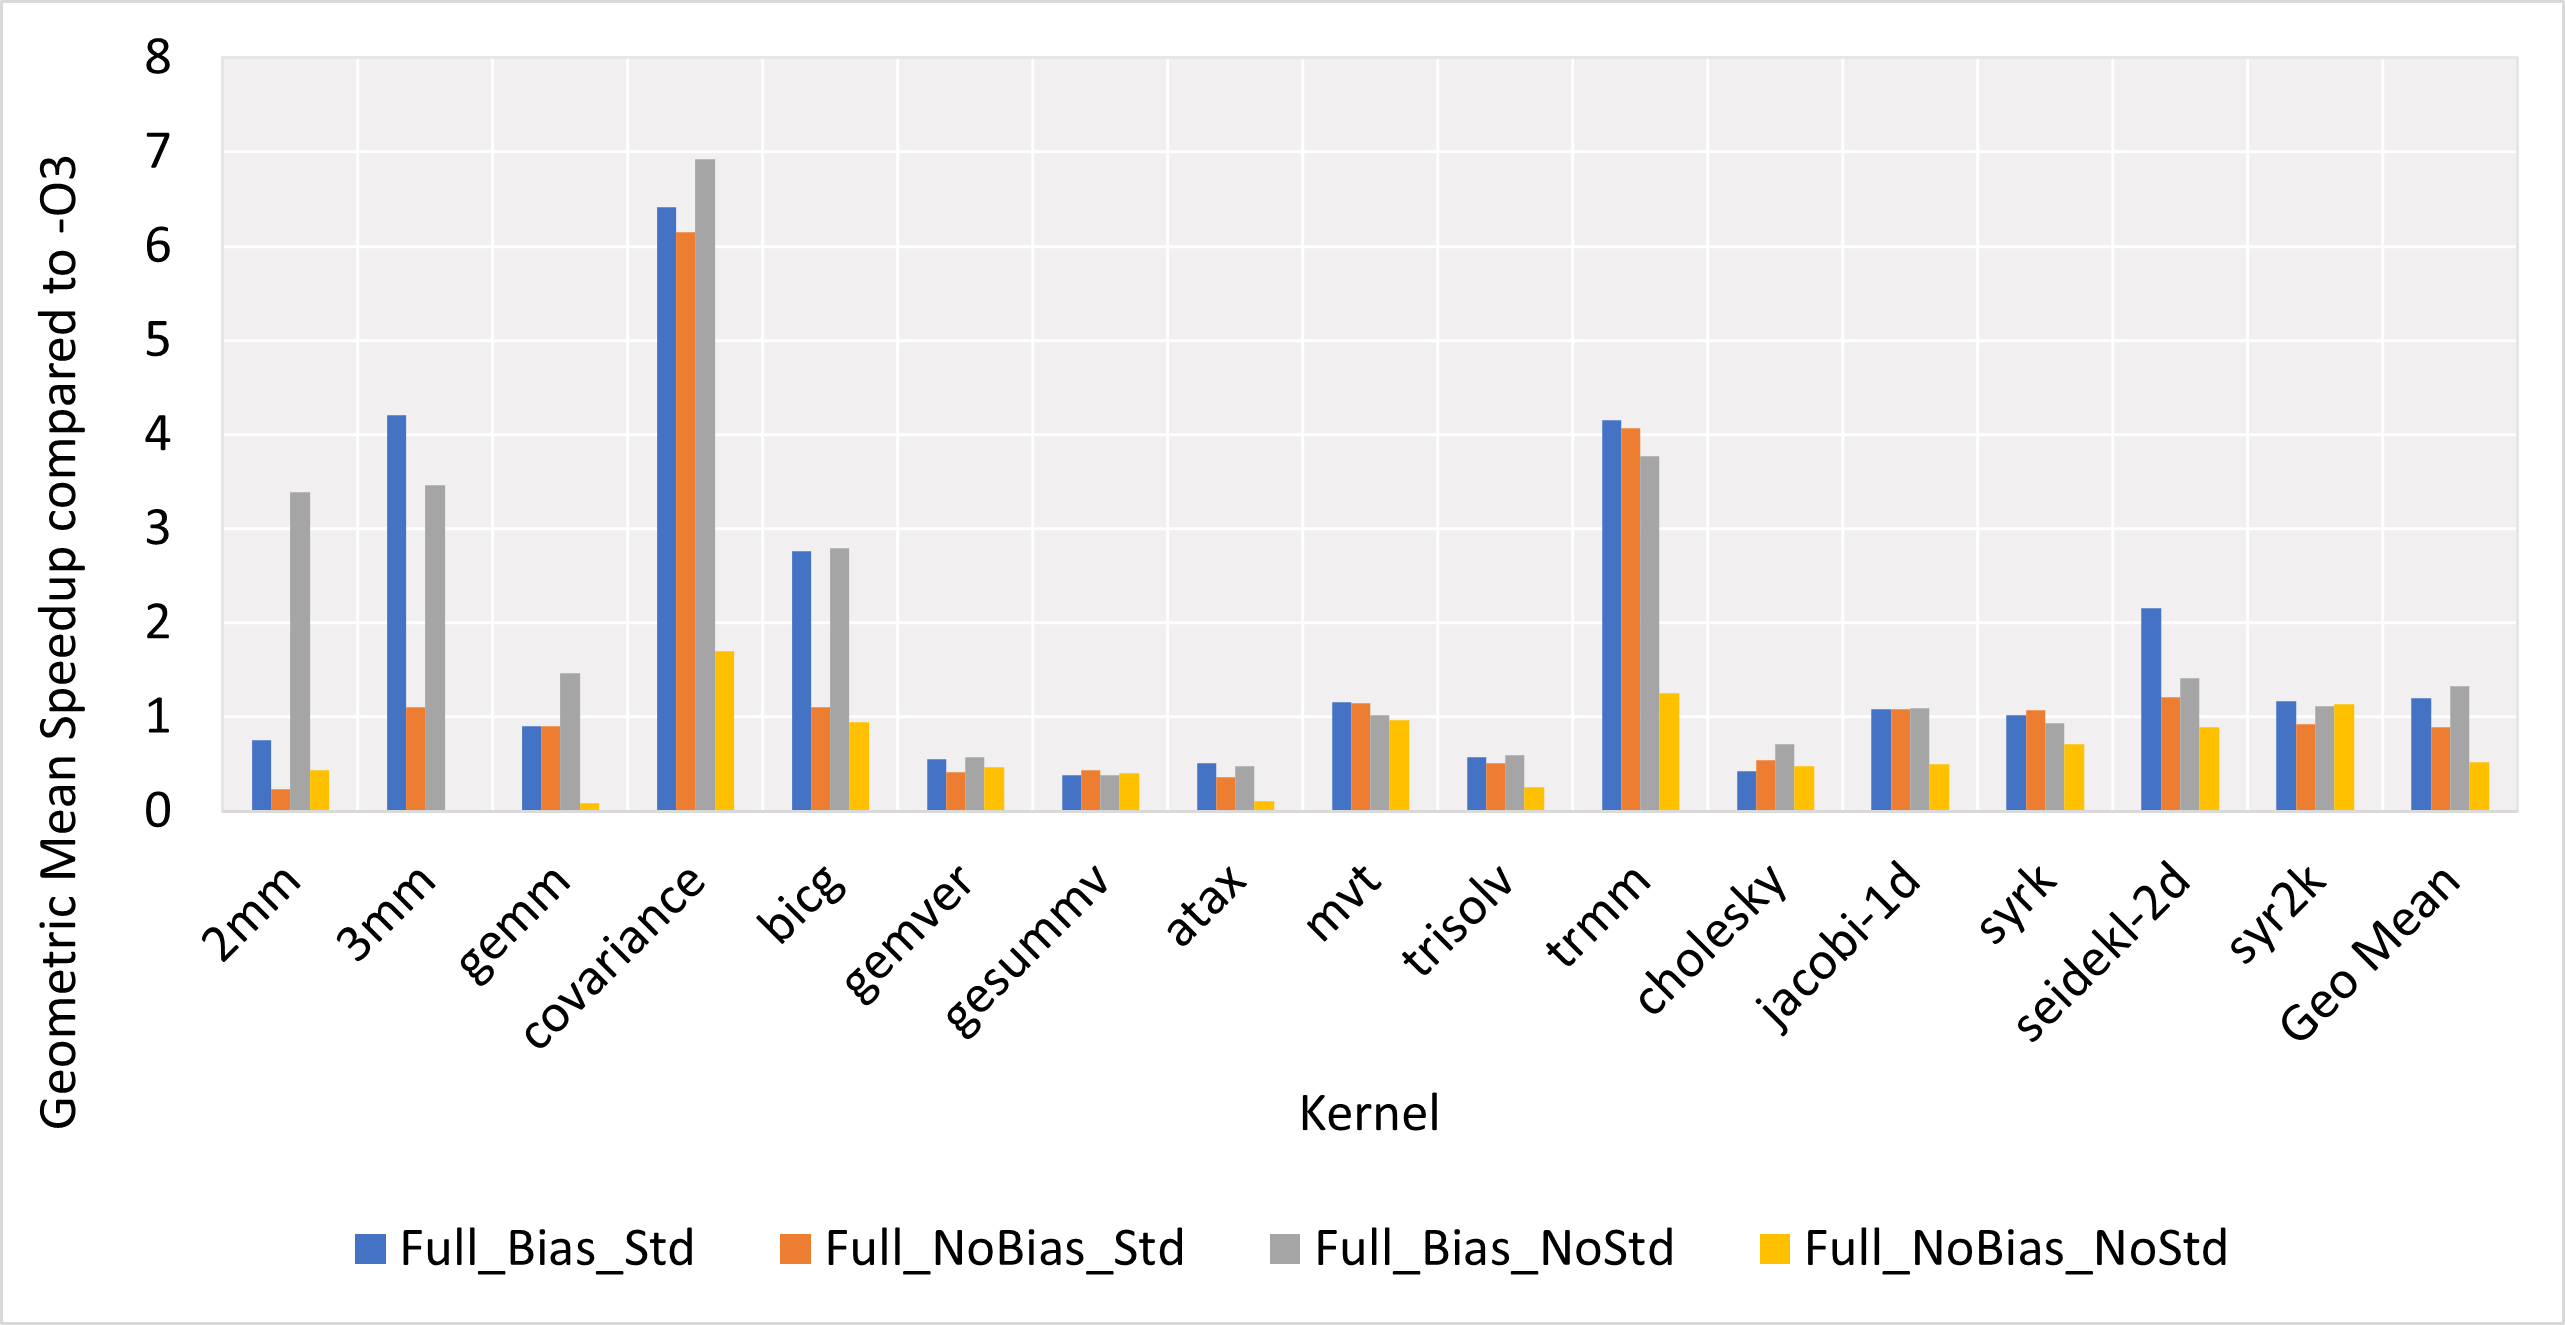
\includegraphics[width=\linewidth]{Images/NoSimple_Chart.png}
  \captionof{figure}{Full Representation}
  \label{NoSimple_Chart}
\end{minipage}
\State{Comparison of PolyGymRL Results for Simple and Full Representation}
\end{figure}

\begin{figure}
\centering
\begin{minipage}{.45\linewidth}
  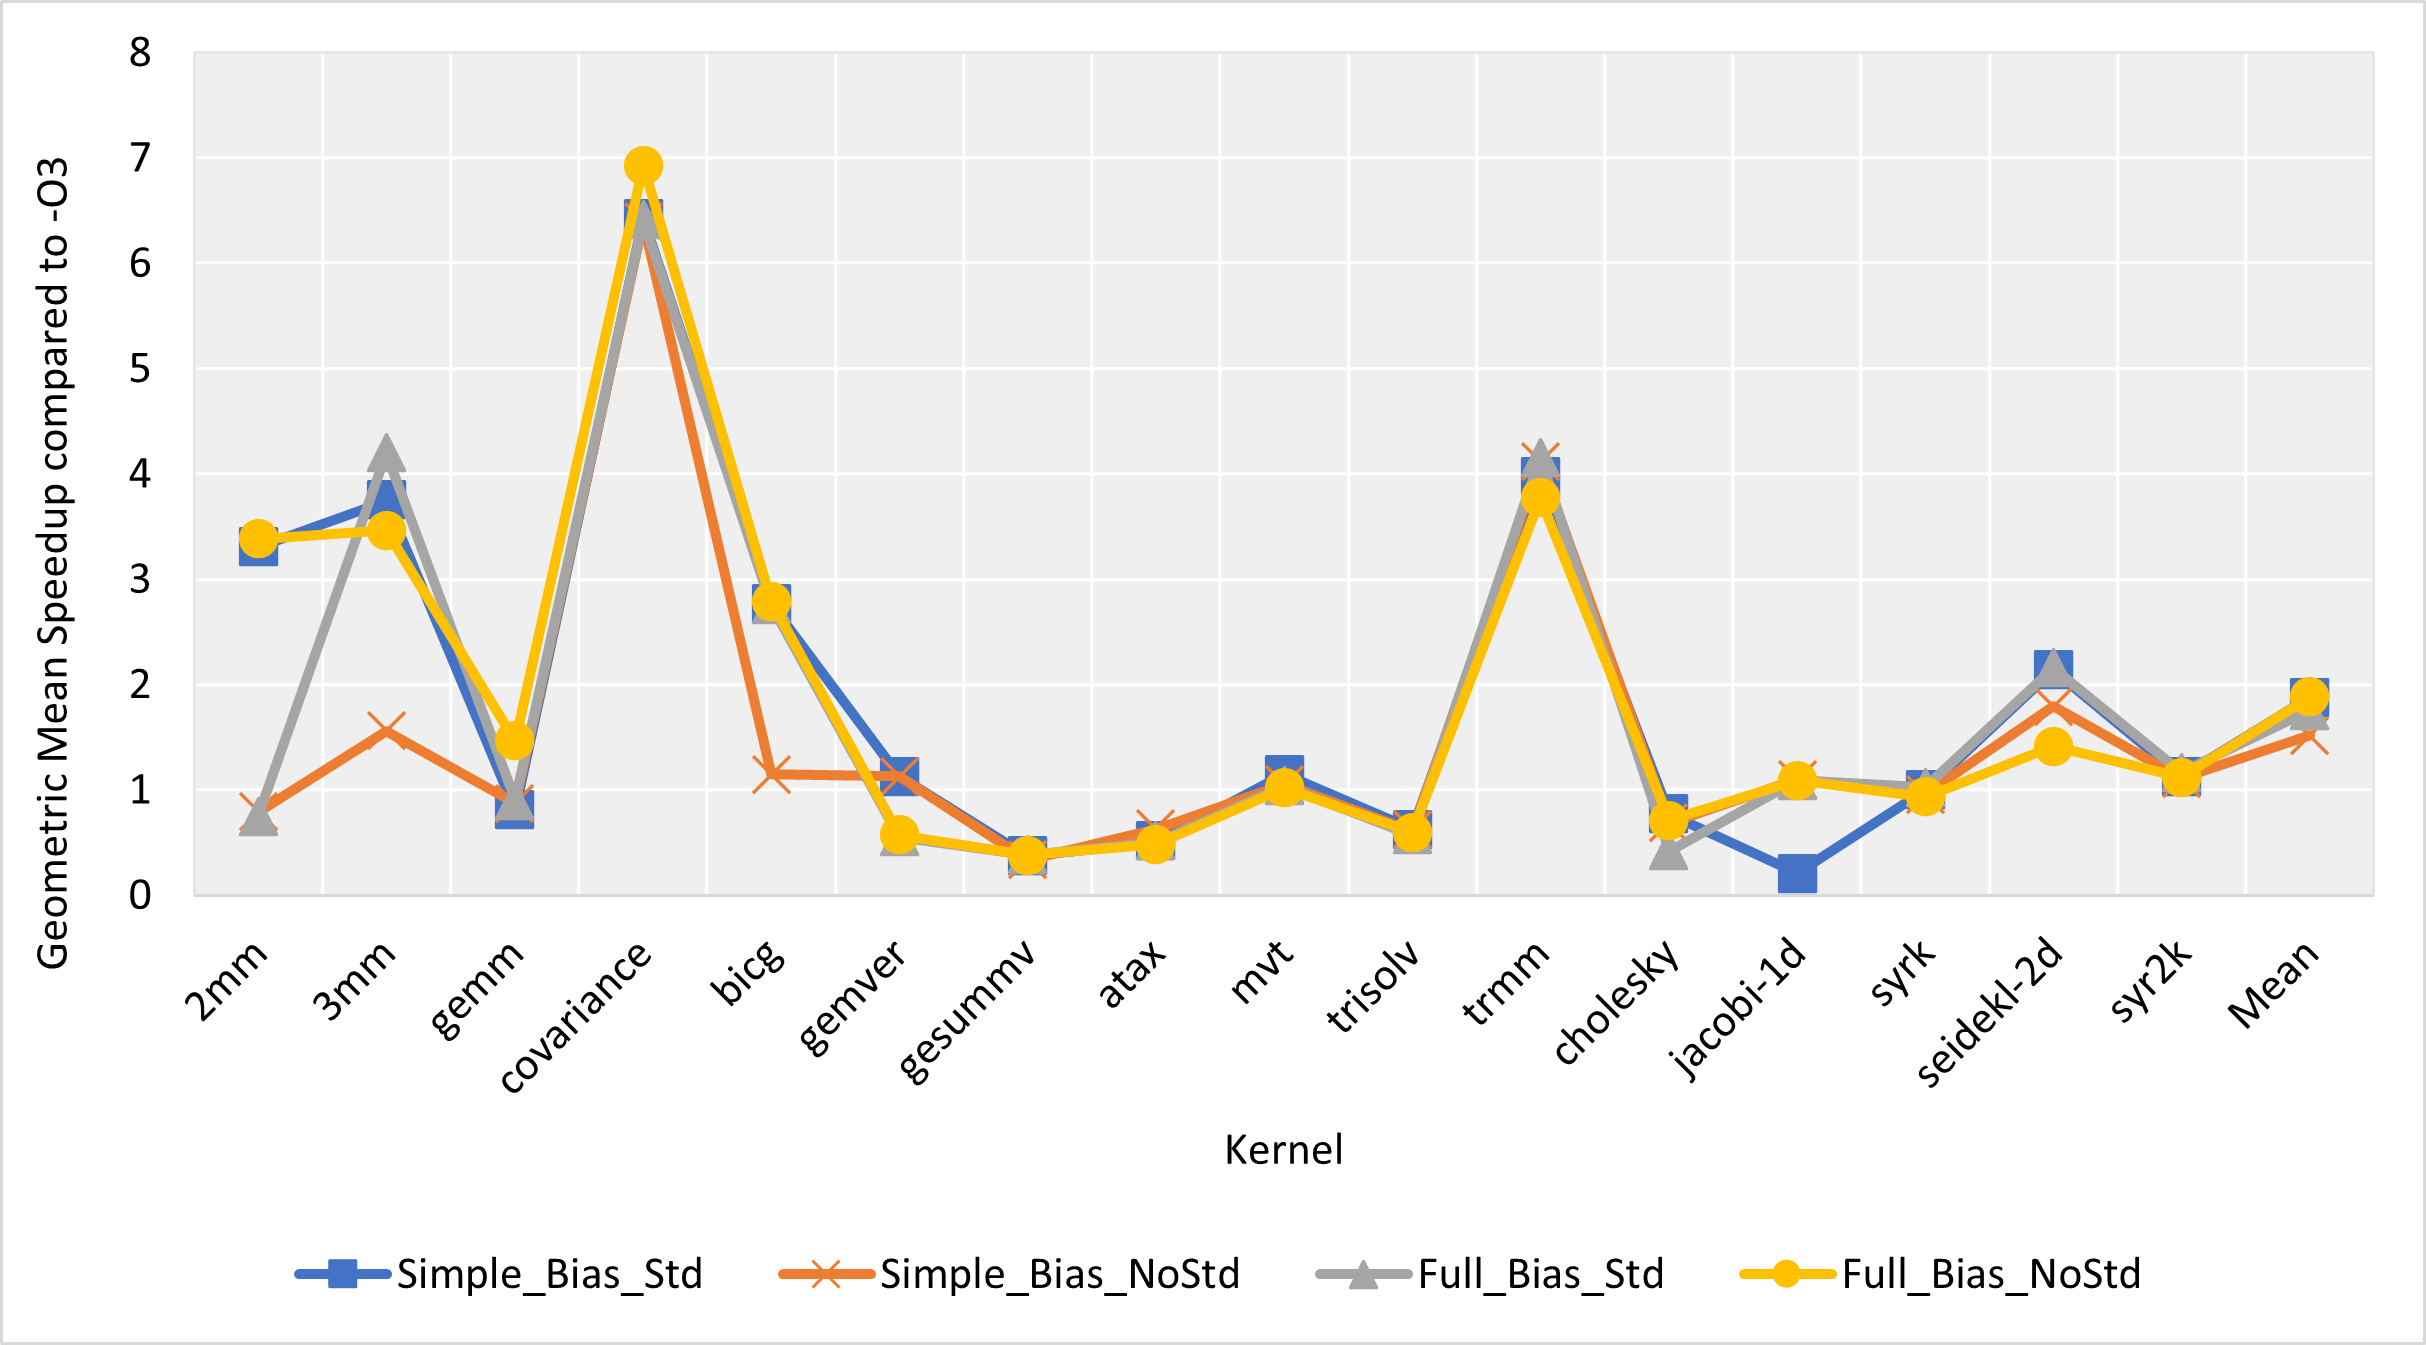
\includegraphics[width=\linewidth]{Images/Bias_Chart.png}
  \captionof{figure}{With Bias}
  \label{Bias_Chart}
\end{minipage}
\hspace{.05\linewidth}
\begin{minipage}{.45\linewidth}
  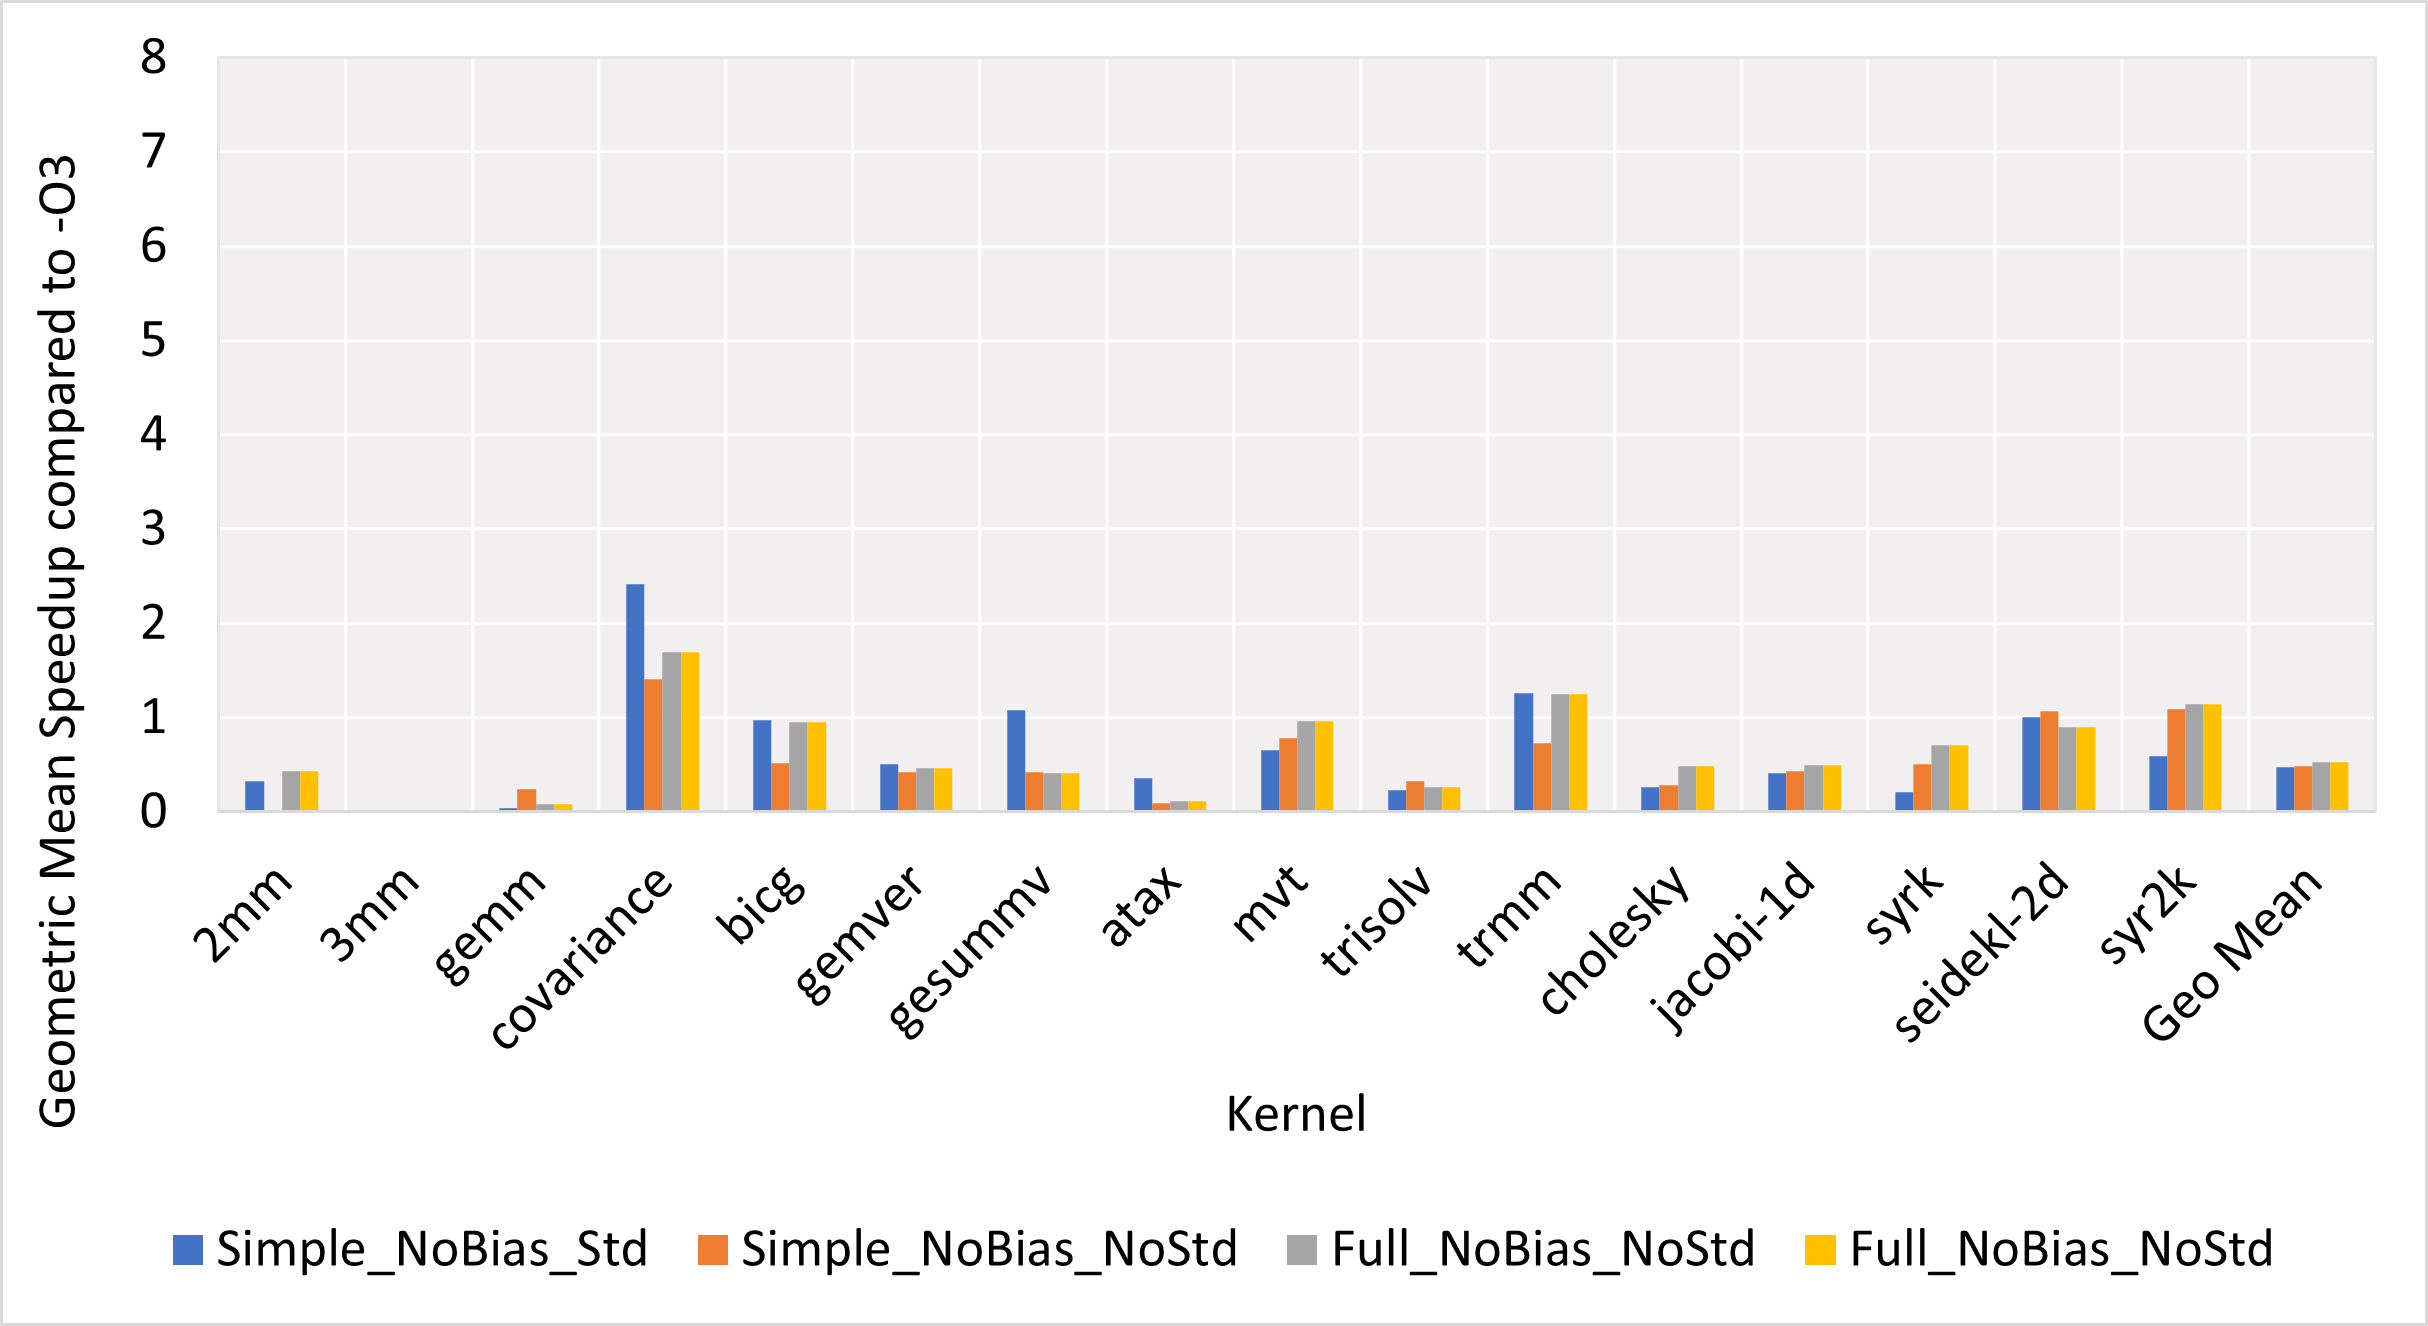
\includegraphics[width=\linewidth]{Images/NoBias_Chart.png}
  \captionof{figure}{Without Bias}
  \label{NoBias_Chart}
\end{minipage}
\State{Comparison of PolyGymRL Results with and without bias while selecting coefficients}
\end{figure}

\begin{figure}
\centering
\begin{minipage}{.45\linewidth}
  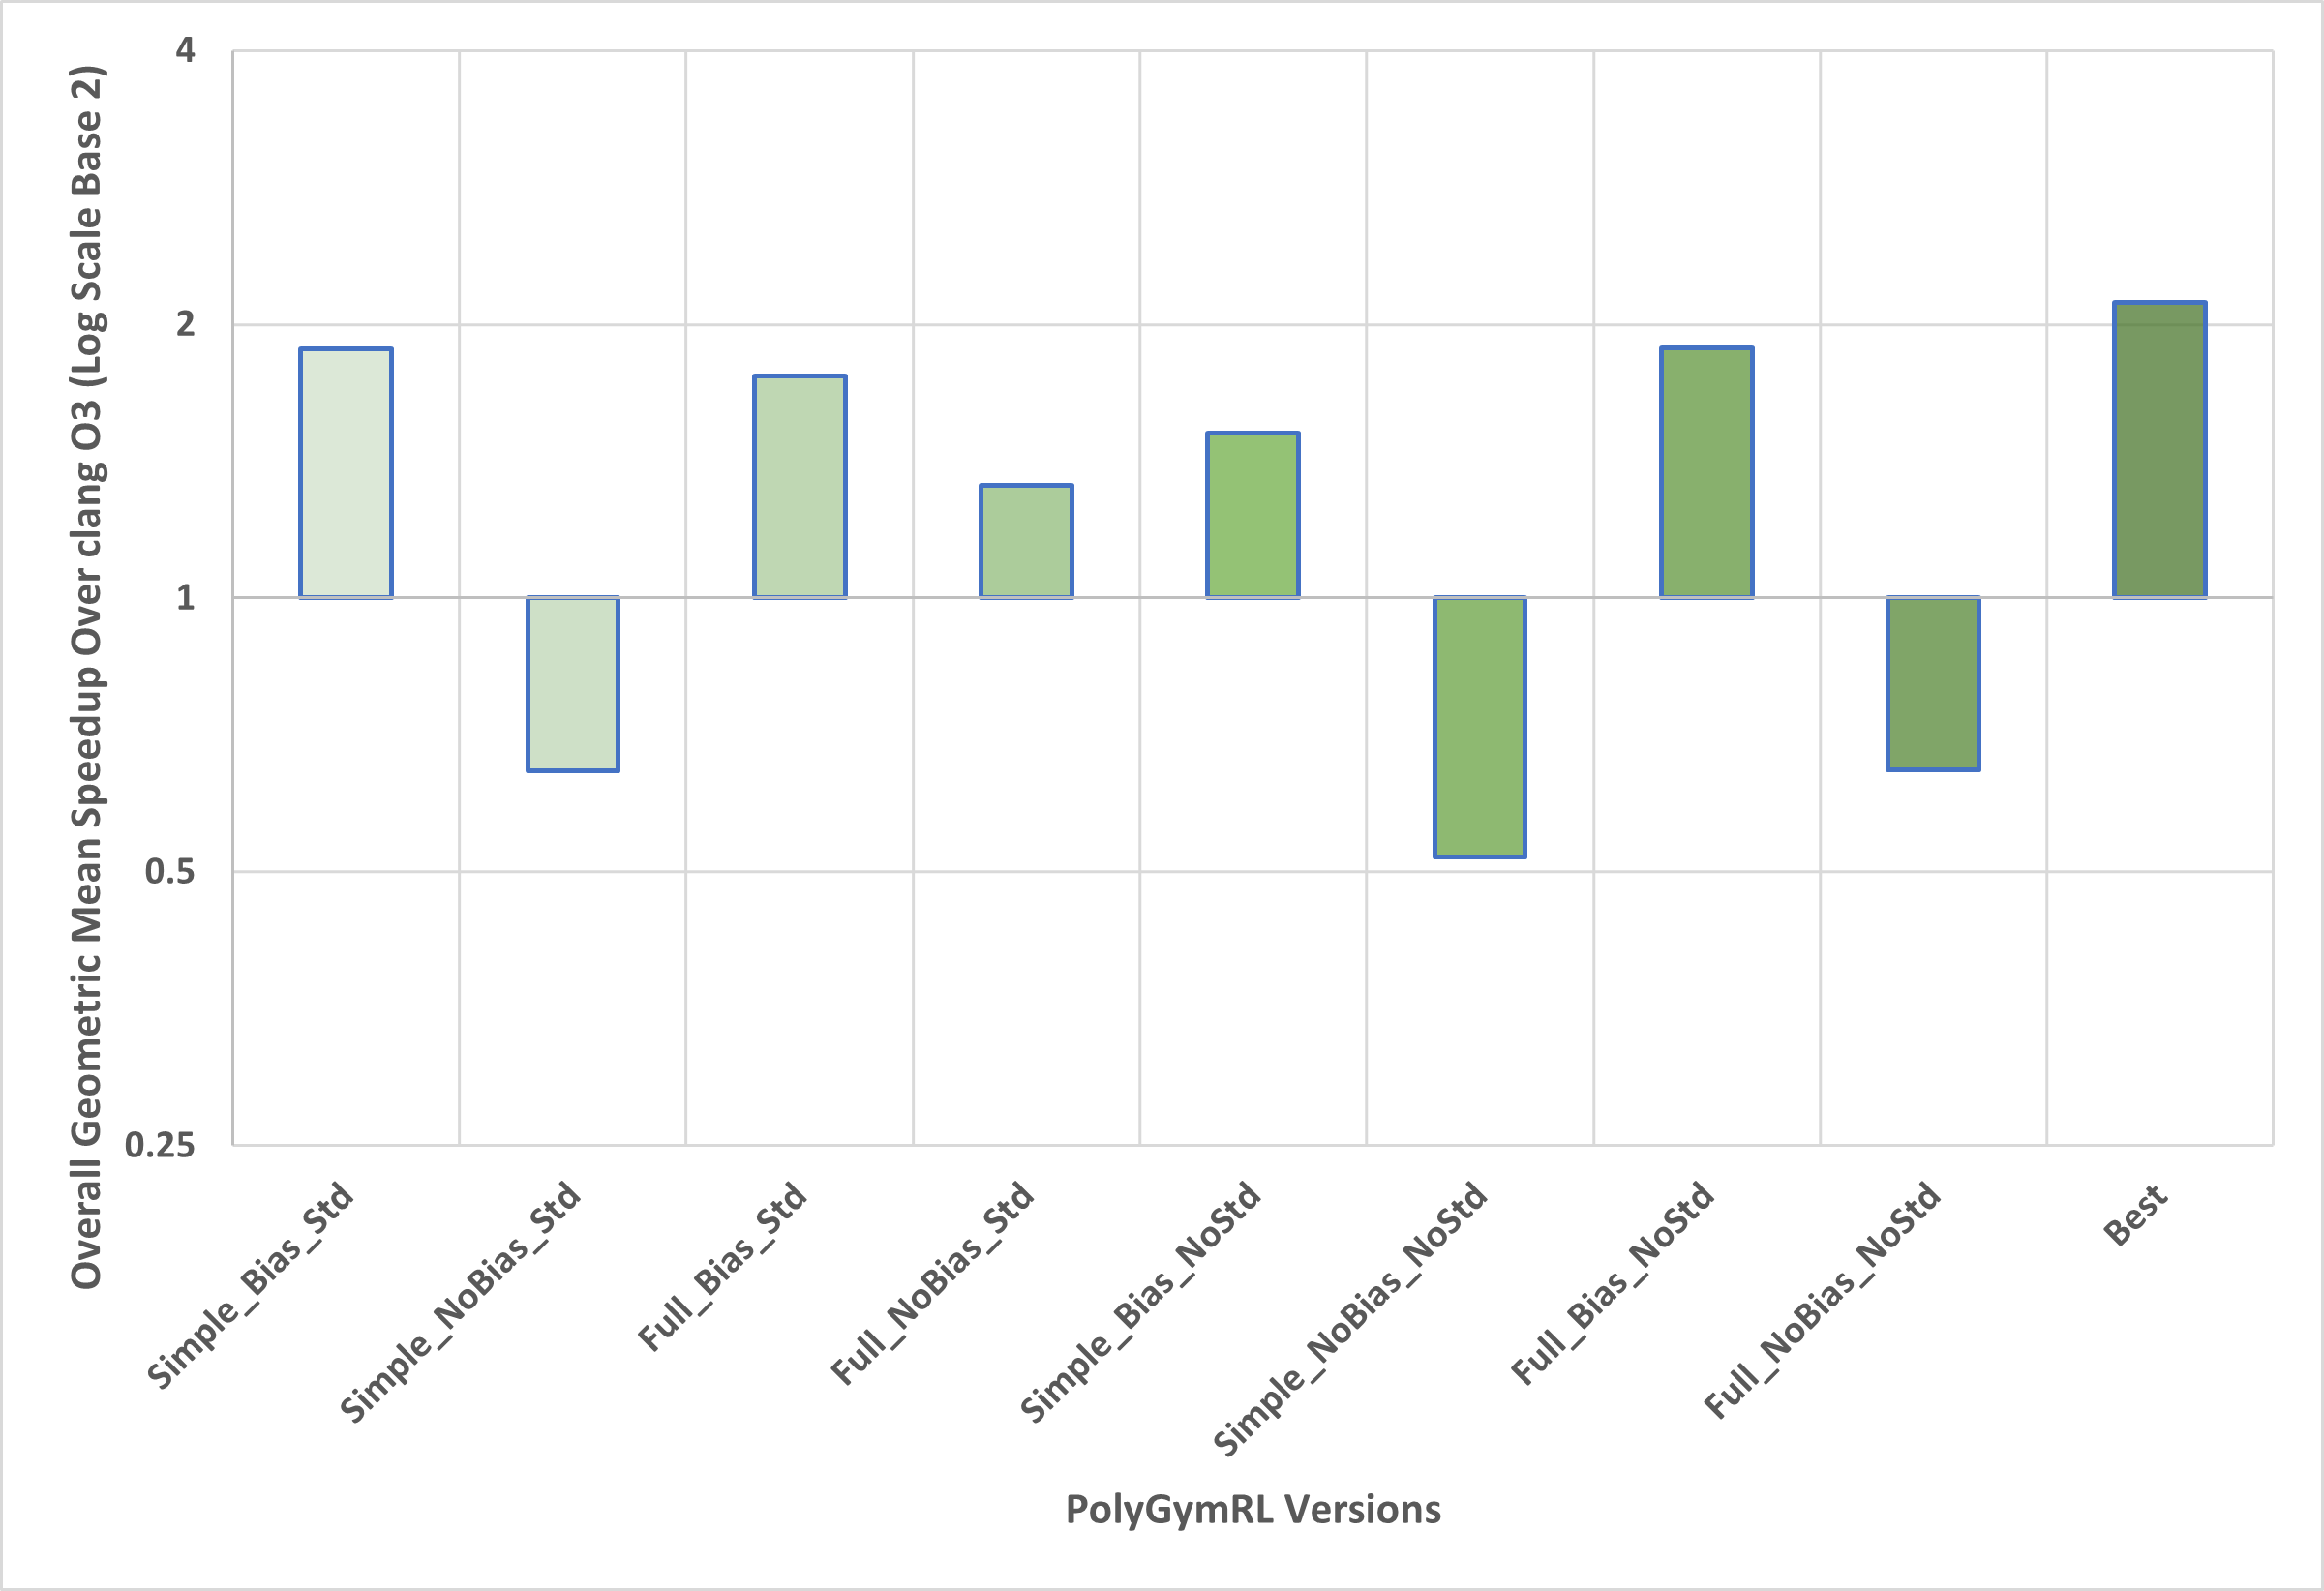
\includegraphics[width=\linewidth]{Images/PolyGymRL_Versions.png}
  \captionof{figure}{Comparison of Speedup for different PolyGymRL Versions}
  \label{PolyGymRL_Versions}
\end{minipage}
\hspace{.05\linewidth}
\begin{minipage}{.45\linewidth}
  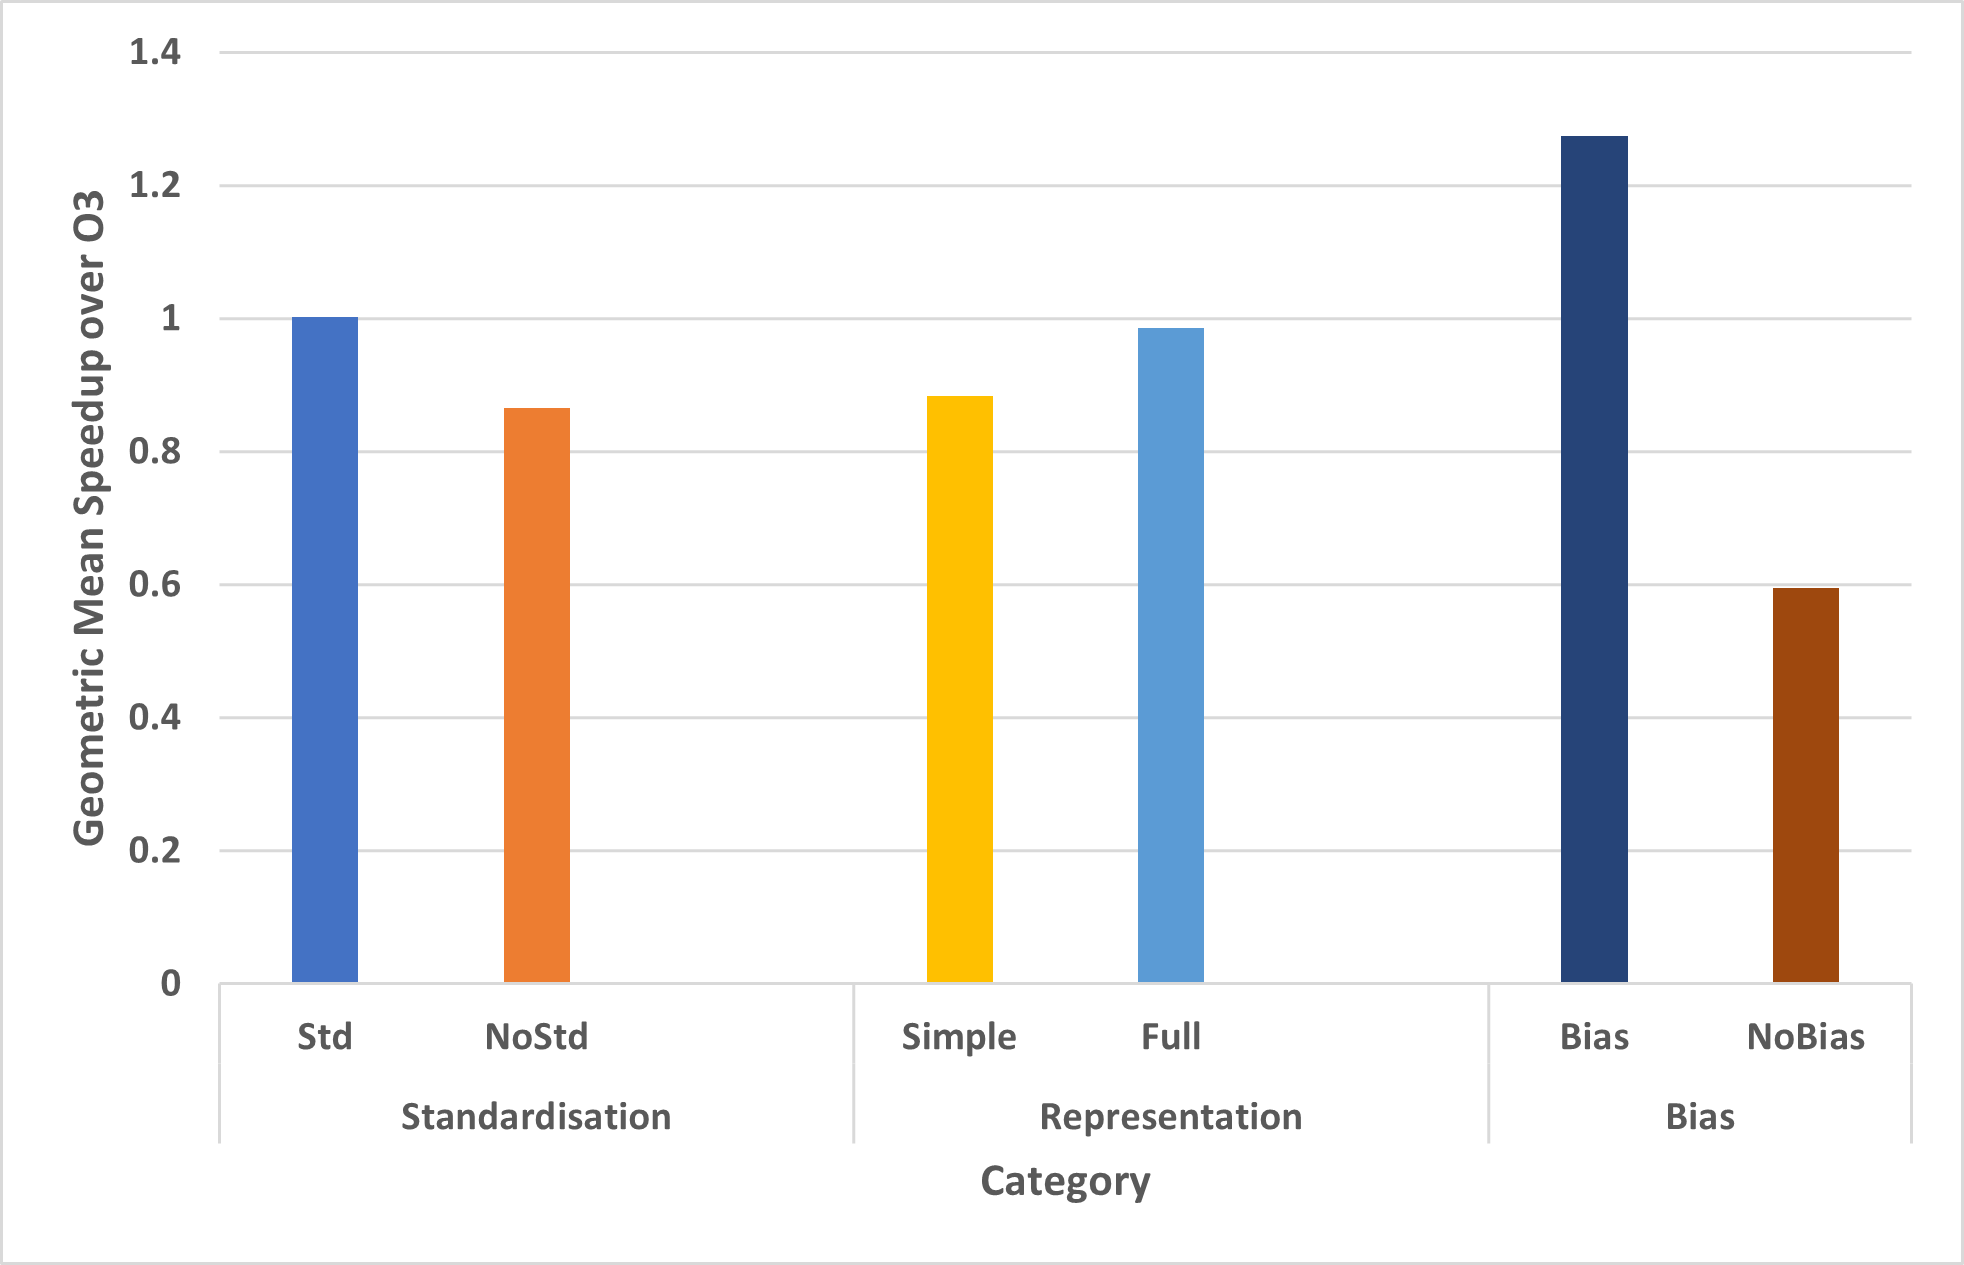
\includegraphics[width=\linewidth]{Images/PolyGymRL_Strategies.png}
  \captionof{figure}{Comparison of Speedup for different PolyGymRL Strategies}
  \label{PolyGymRL_Strategies}
\end{minipage}
\end{figure}

\begin{figure}[htbp]
  \centering
  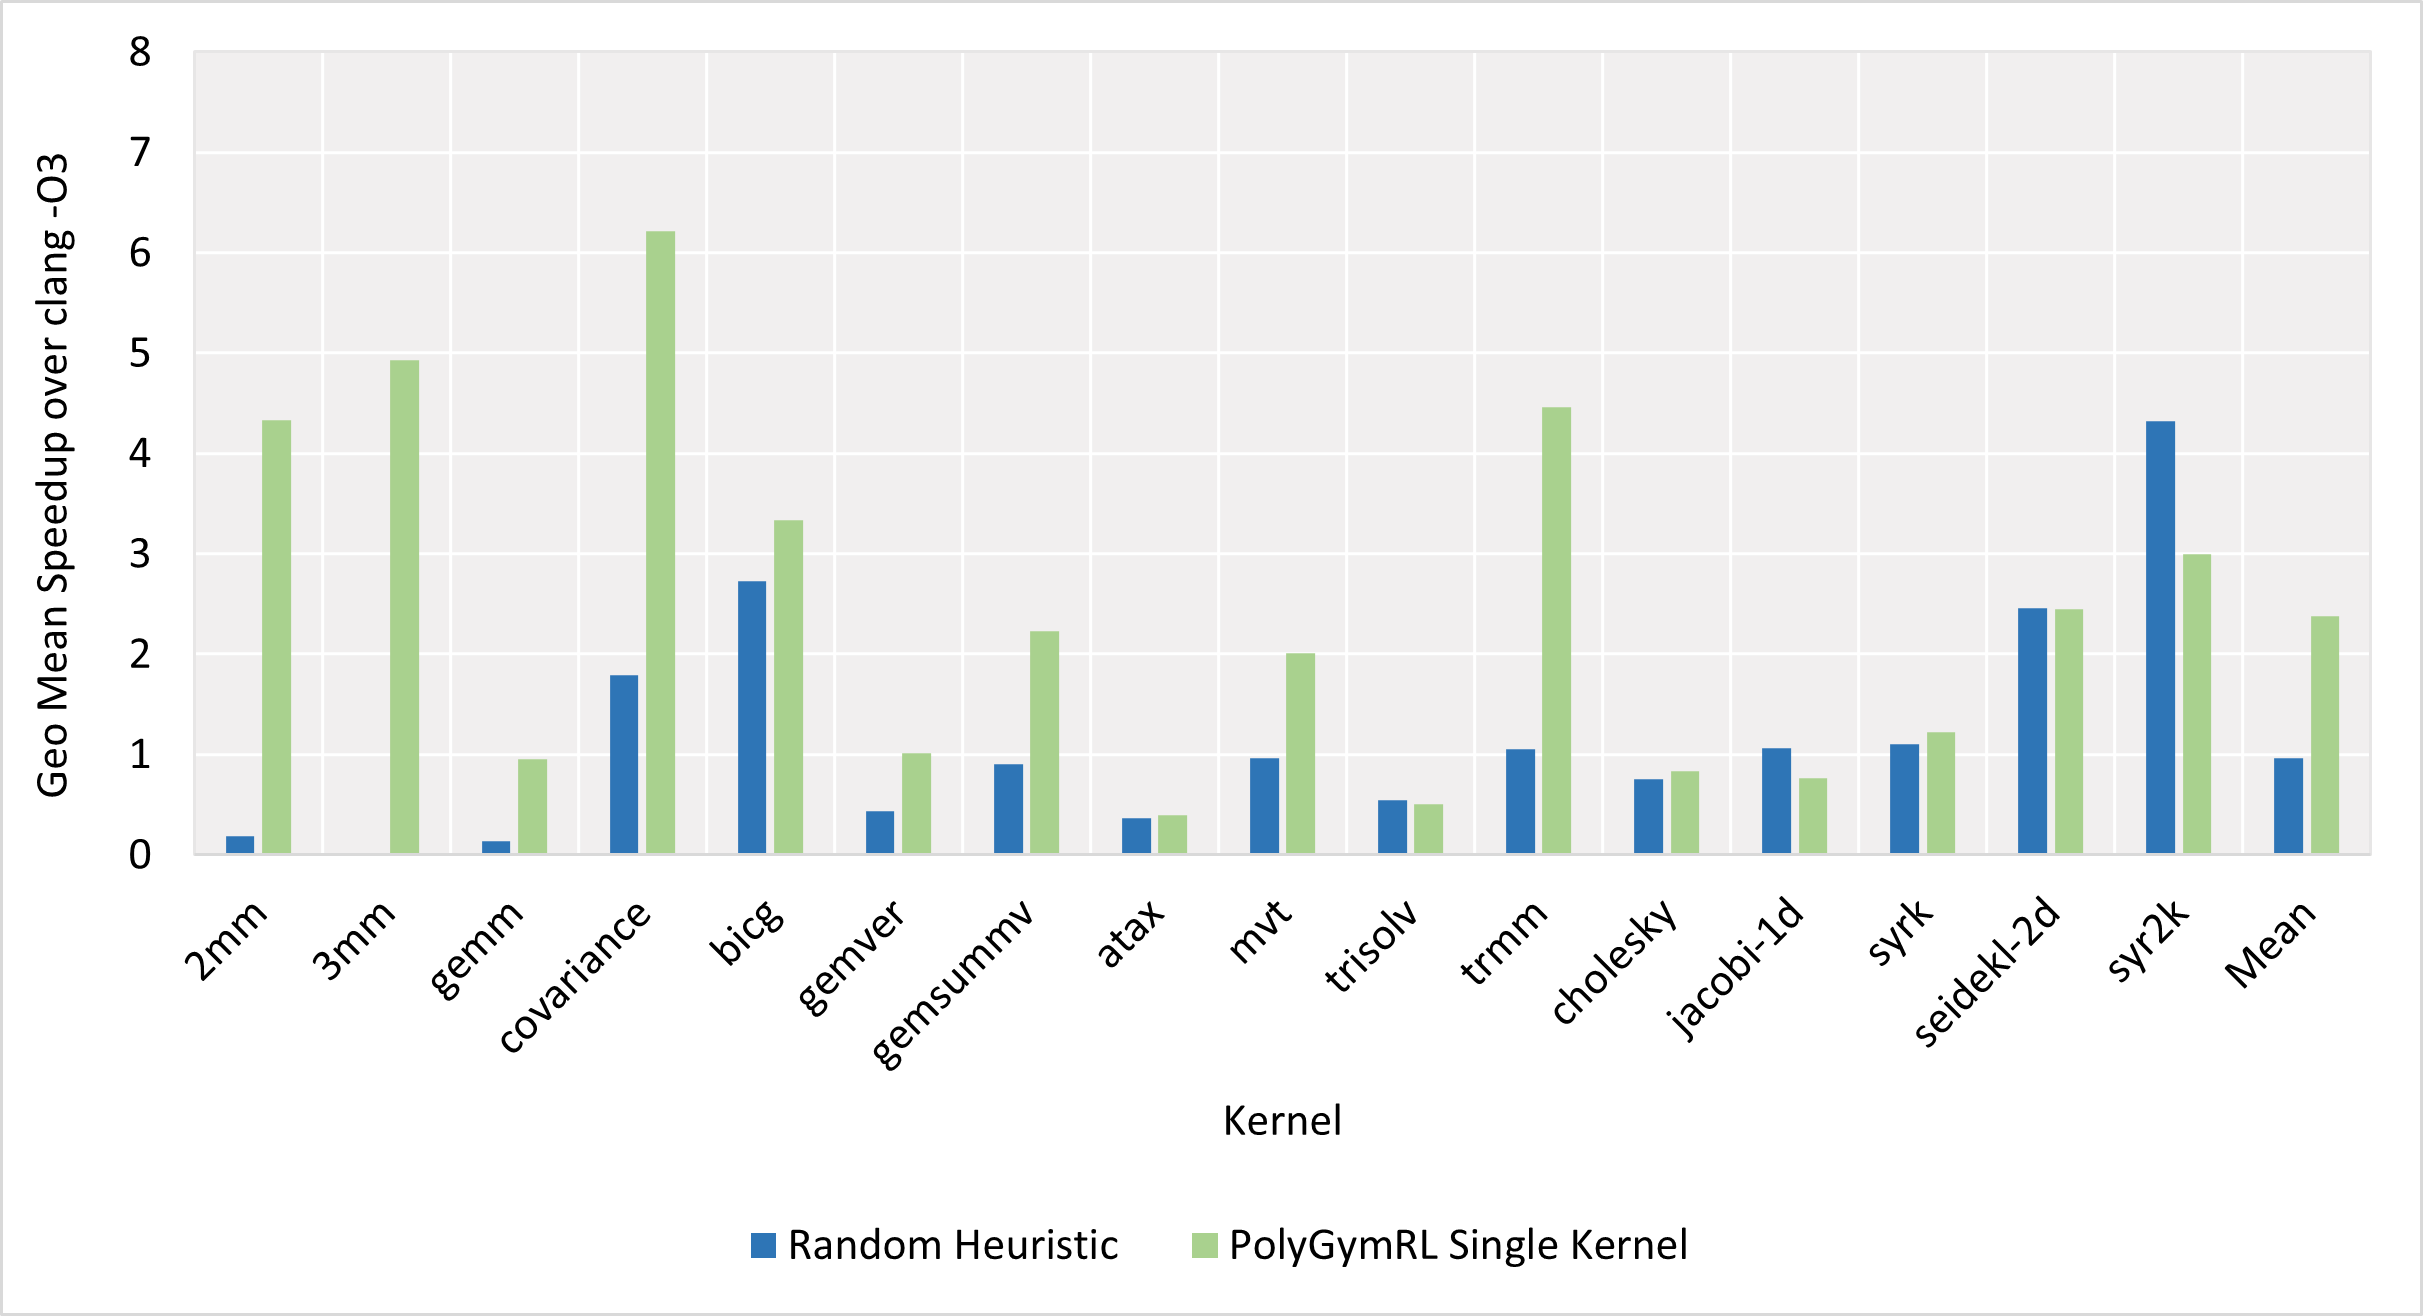
\includegraphics[width=0.75\textwidth]{Images/Chart_Single_PolyGym_PolyGymRL.png}    
  \caption{Comparison of Average Speedup achieved in PolyGym and PolyGymRL while training and testing on the same kernel}
  \label{fig:single_PolyGym_PolyGymRL}
\end{figure}

\begin{figure}[htbp]
  \centering
  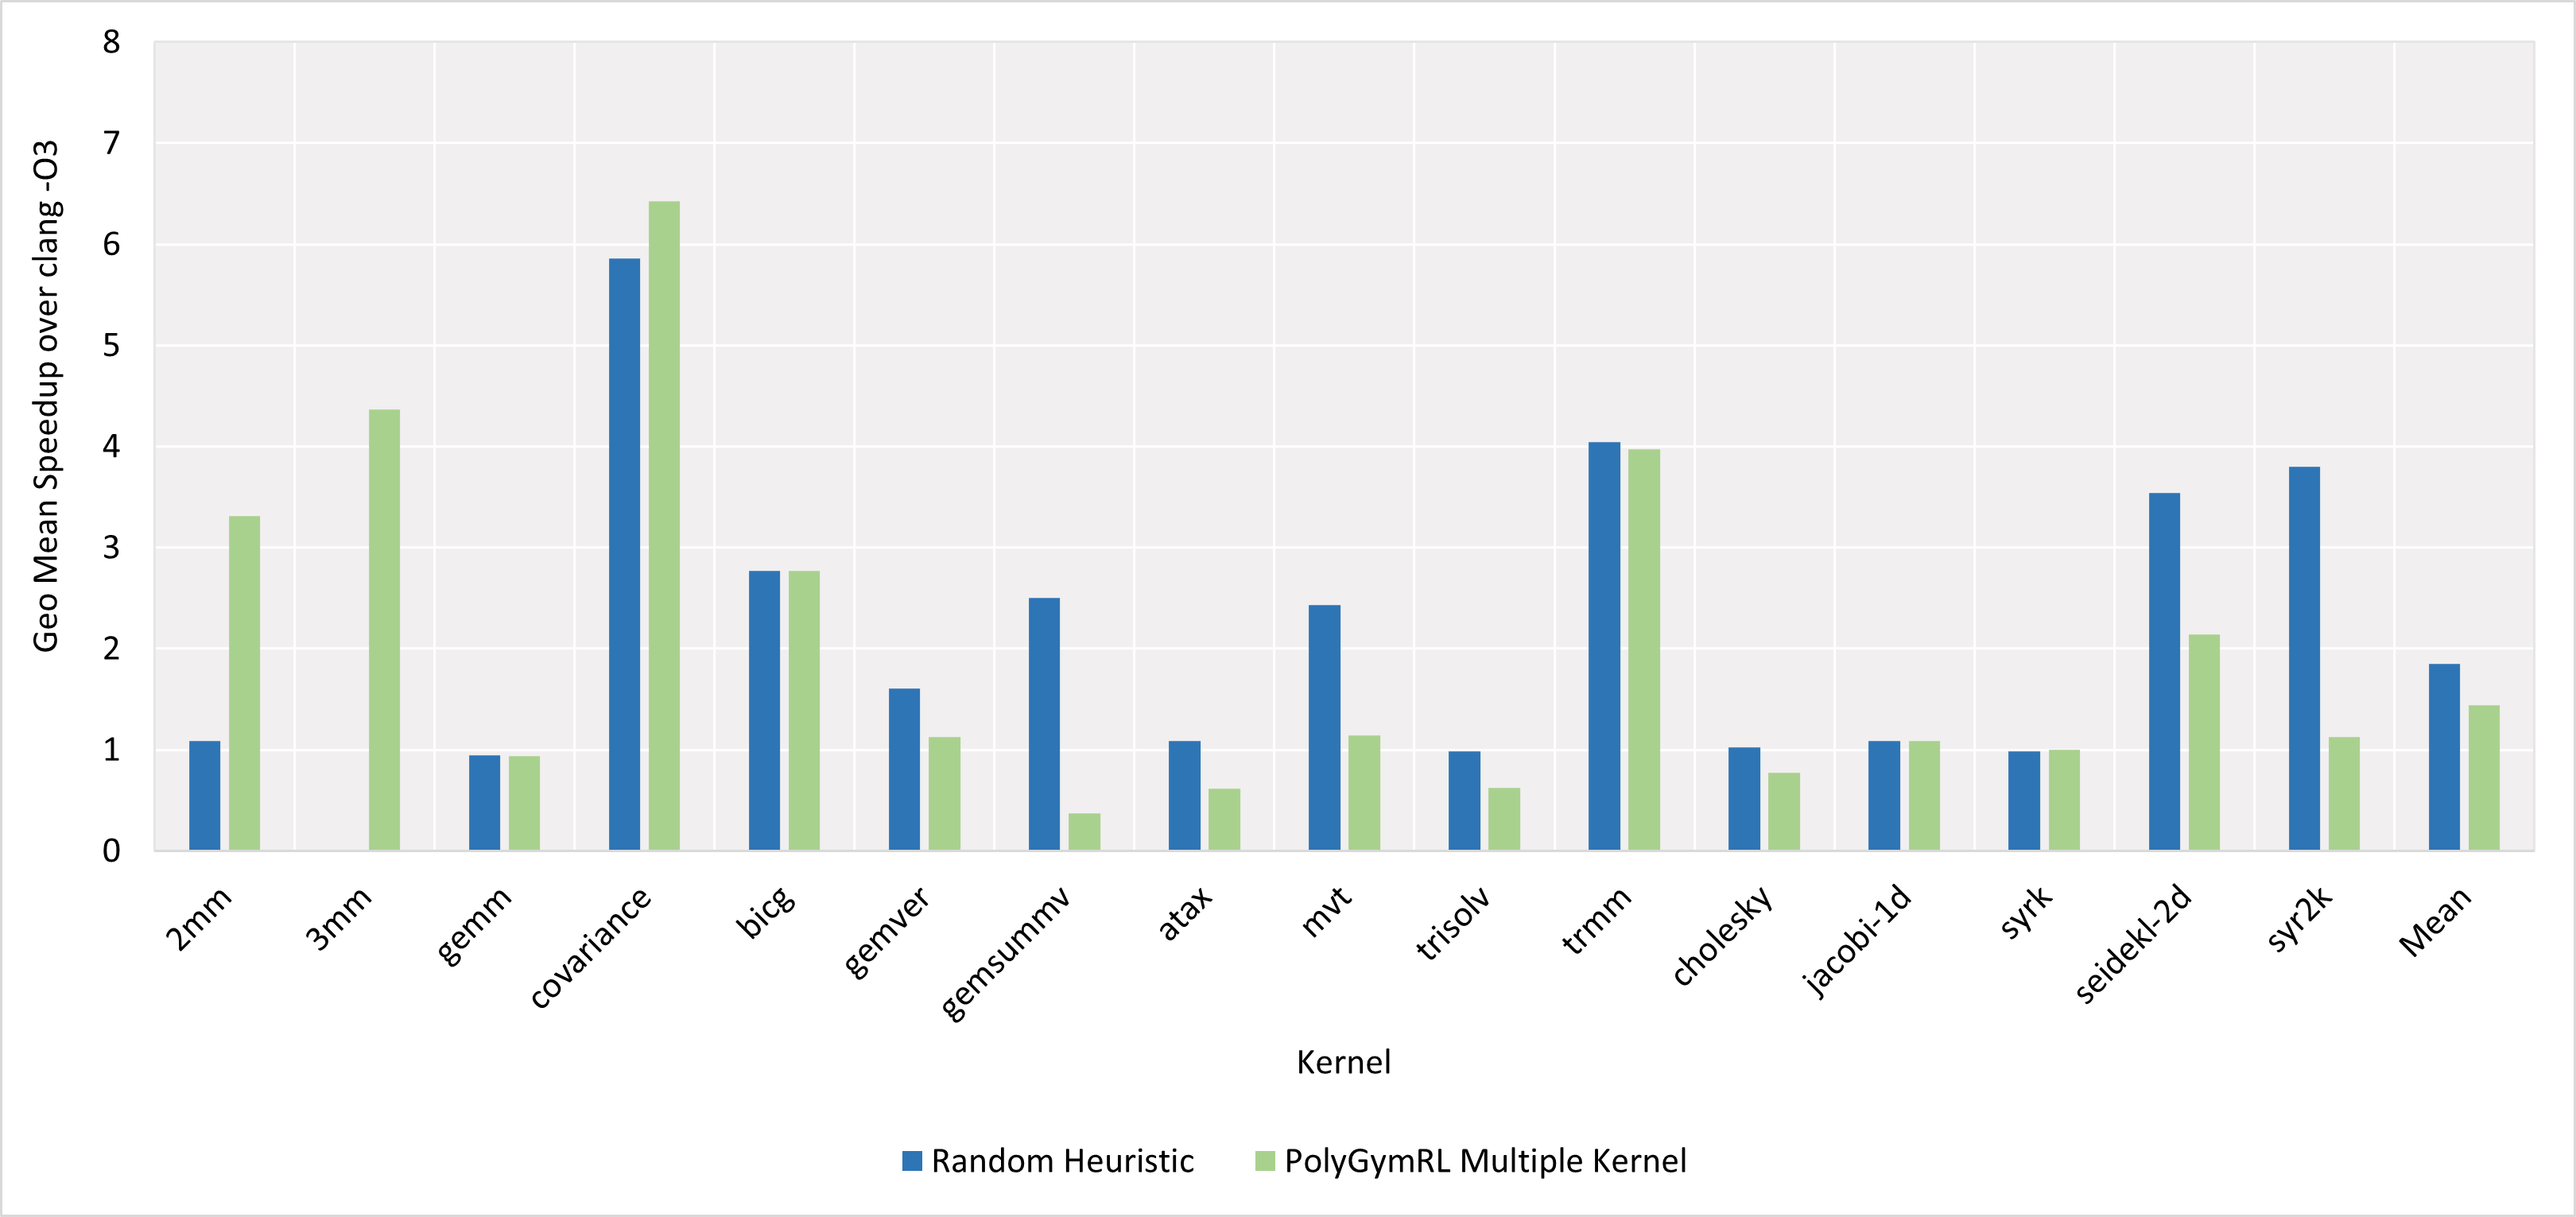
\includegraphics[width=0.75\textwidth]{Images/Chart_Multiple_PolyGym_PolyGymRL.png}    
  \caption{Comparison of Average Speedup achieved in PolyGym and PolyGymRL using Leave-One-Out Evaluation}
  \label{fig:multi_PolyGym_PolyGymRL}
\end{figure}
 




% You may delete everything from \appendix up to \end{document} if you don't need it.
\appendix

\chapter{Results}



\section{PolyGymRL Results}

\begin{figure}[htbp]
  \centering
  \includegraphics[width=0.95\textwidth]{Images/BenchMarking.png}    
  \caption{Result Data for PolyGymRL}
  \label{fig:BenchMarking}
\end{figure}

\section{Comparison of PolyGym and PolyGymRL}

\begin{figure}
\centering
\begin{minipage}{.45\linewidth}
  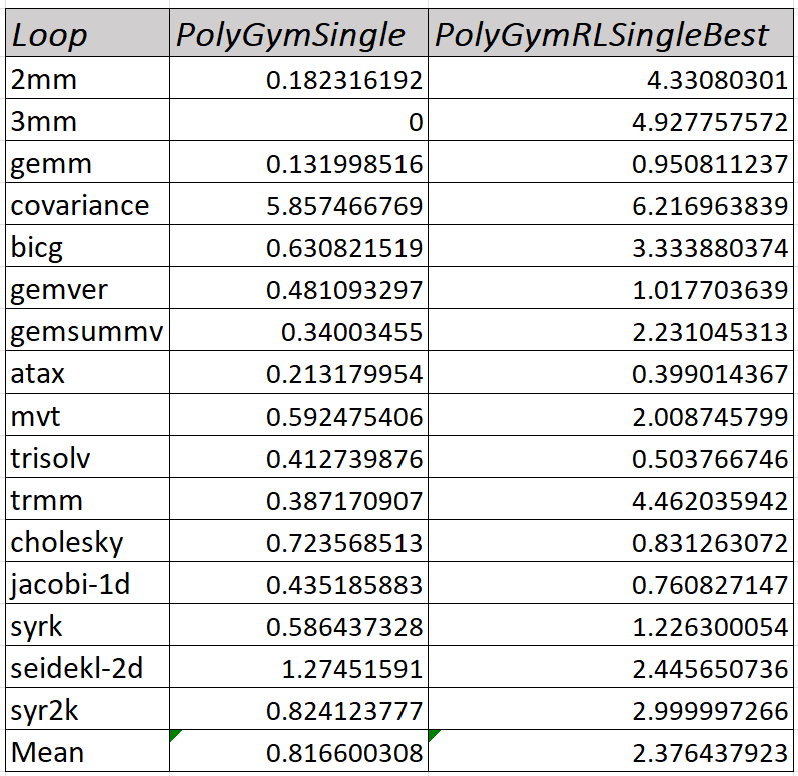
\includegraphics[width=\linewidth]{Images/Benchmarking_Single.png}
  \captionof{figure}{Results of PolyGym and PolyGymRL for single kernel}
  \label{Benchmarking_Single}
\end{minipage}
\hspace{.05\linewidth}
\begin{minipage}{.45\linewidth}
  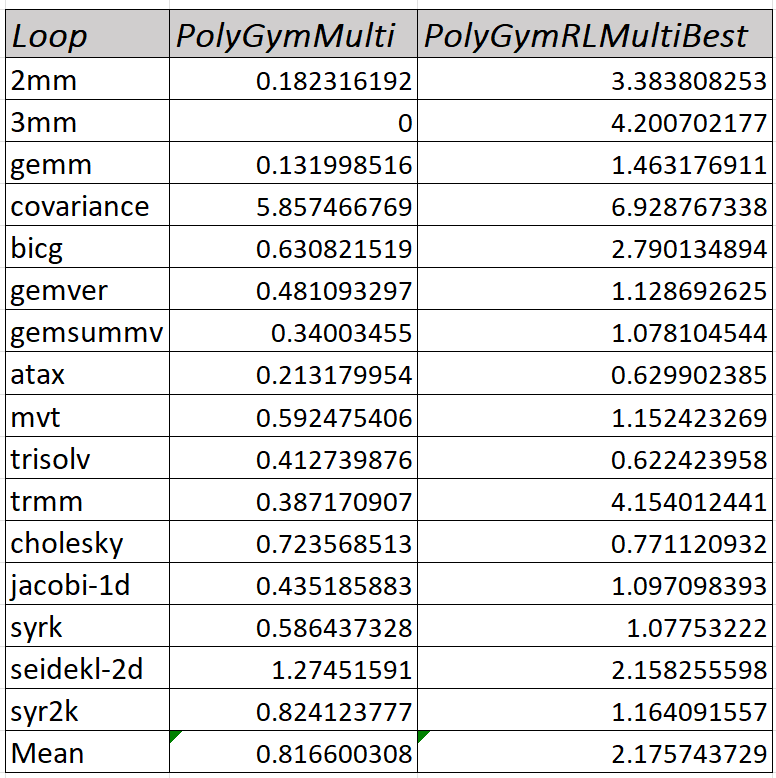
\includegraphics[width=\linewidth]{Images/Benchmarking_Multiple.png}
  \captionof{figure}{Results of PolyGym and PolyGymRL for multiple kernels}
  \label{Benchmarking_Multiple}
\end{minipage}
\State{Results Comparison of PolyGym and PolyGymRL for single and multiple kernels}
\end{figure}



\end{document}
